\documentclass[10pt,a4paper]{article}
\usepackage[margin=1.8cm]{geometry}
\usepackage{graphicx,booktabs,float,caption,hyperref,enumitem}
\captionsetup{font=small,labelfont=bf}
\setlist{nosep,leftmargin=1.2em}
\setlength{\parskip}{3pt}\setlength{\parindent}{0pt}
\graphicspath{{../results/figures/}}
\begin{document}
\begin{center}
{\Large\bfseries Homework 1: Image Enhancement}\\[2pt]
Computer Vision, Fall 2026 \quad|\quad Nuras Assylbekov (matricola VR565535)\\
Code and data: \textbf{[REPOSITORY LINK]}
\end{center}

\section*{1. Objective, images and sources}
We build a small, reproducible pipeline that enhances images with low contrast, non-uniform illumination and noise, using only classical methods (OpenCV, NumPy; scikit-image only for SSIM; no neural networks). We compare four approaches, plus one extra variant, with fixed data and fixed parameters, quantitatively (PSNR, SSIM, MAE) and qualitatively.

\textbf{Images (5, own photographs).} \emph{board1--board3}: a classroom whiteboard with handwriting under strong, patchy sunlight and shadows (non-uniform illumination, thin strokes that are hard to see). \emph{room\_dark}: an indoor scene in very low light. \emph{night\_street}: a night scene seen through a window, with glare and reflections. All were taken by the author with a phone (November 2026), have no third-party licence restrictions (own work) and are included in the repository; images are resized to 1024\,px on the long side.

\textbf{Synthetic degradation and the role of the reference.} Each original $I$ is degraded as $I_d = 127.5 + 0.45\,(I-127.5) + \mathcal N(0,6^2)$, clipped to $[0,255]$, with a fixed seed (42 + image index). The originals serve as references for the metrics. In real-world scenarios a clean reference is generally not available, and here the ``reference'' is itself unevenly lit (or dark and noisy), so the metrics measure fidelity to the original, not an ideal enhancement.

\section*{2. Methods and parameters}
All methods are applied to $I_d$. Colour images are processed in CIE Lab (OpenCV 8-bit), modifying only the lightness channel $L$ unless stated otherwise.
\begin{enumerate}
\item \textbf{Baseline:} the degraded image, no processing.
\item \textbf{Linear contrast stretching (luminance):} $L' = 255\,(L - L_{min})/(L_{max}-L_{min})$ (min--max, percentiles 0/100); $a,b$ unchanged, so hues are preserved. \emph{Extra variant (RGB*):} the same stretch applied independently to B, G, R, to show colour shifts.
\item \textbf{Histogram equalization:} \texttt{cv2.equalizeHist} on the $L$ channel; $a,b$ unchanged.
\item \textbf{Our method: stretch + non-local means (NLM).} Luminance stretch followed by \texttt{fastNlMeansDenoisingColored} ($h=h_c=6$, template 7, search window 21). Motivation: stretching multiplies the noise by the same gain as the signal, so we denoise afterwards; the price is that NLM may smooth fine details.
\end{enumerate}

\section*{3. Results}
Figures~\ref{fig:b1} and \ref{fig:ns} show original, degraded and processed images for two scenes (all five are in the repository). Table~\ref{tab:m} reports the metrics for every image and method.

\begin{figure}[H]\centering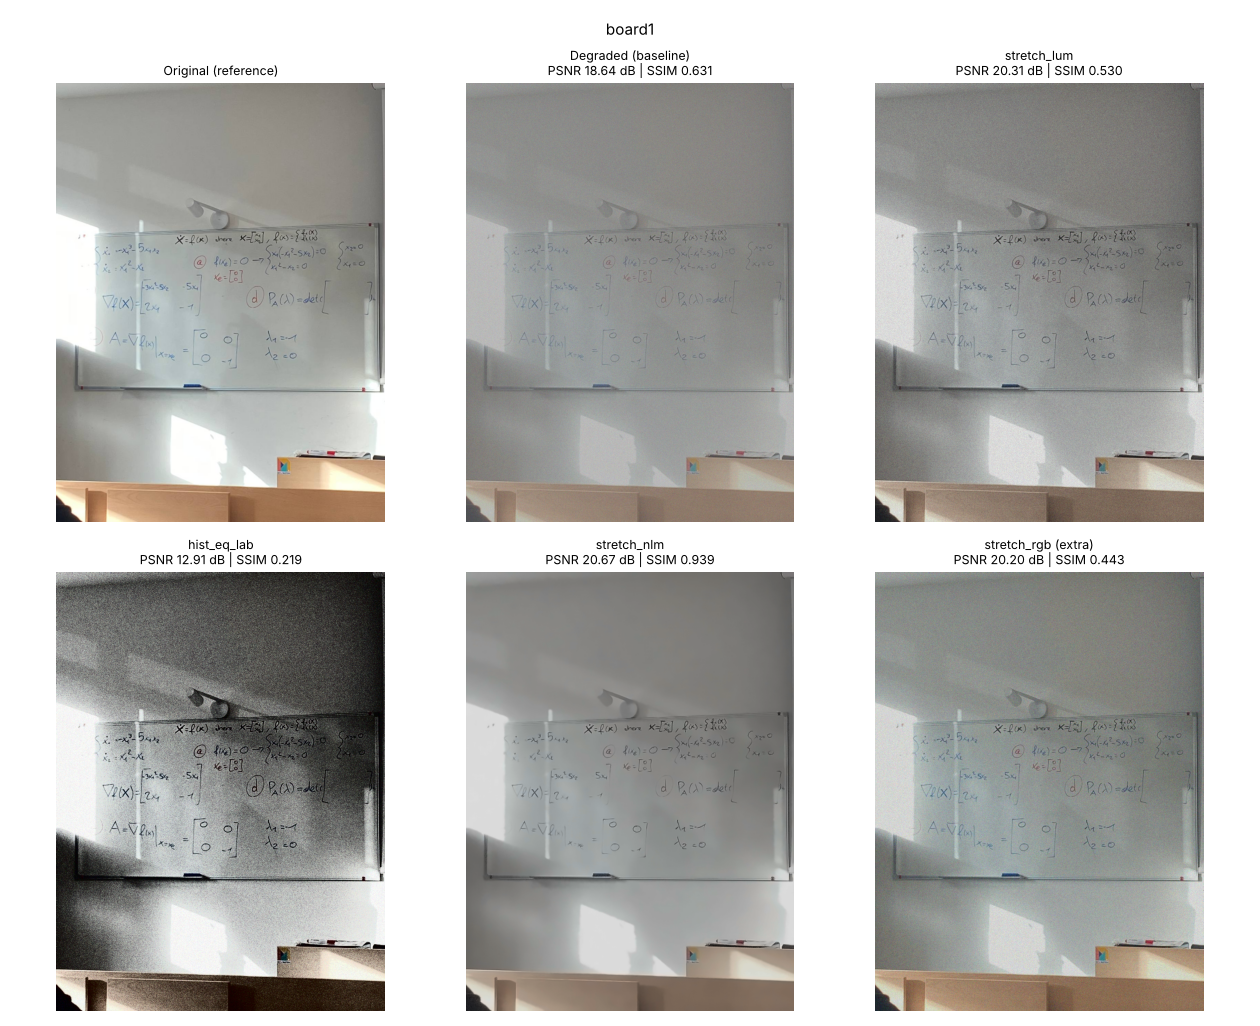
\includegraphics[width=0.84\linewidth]{board1_comparison.png}
\caption{board1: original (reference), degraded baseline and results, with PSNR/SSIM against the original.}\label{fig:b1}\end{figure}

\begin{figure}[H]\centering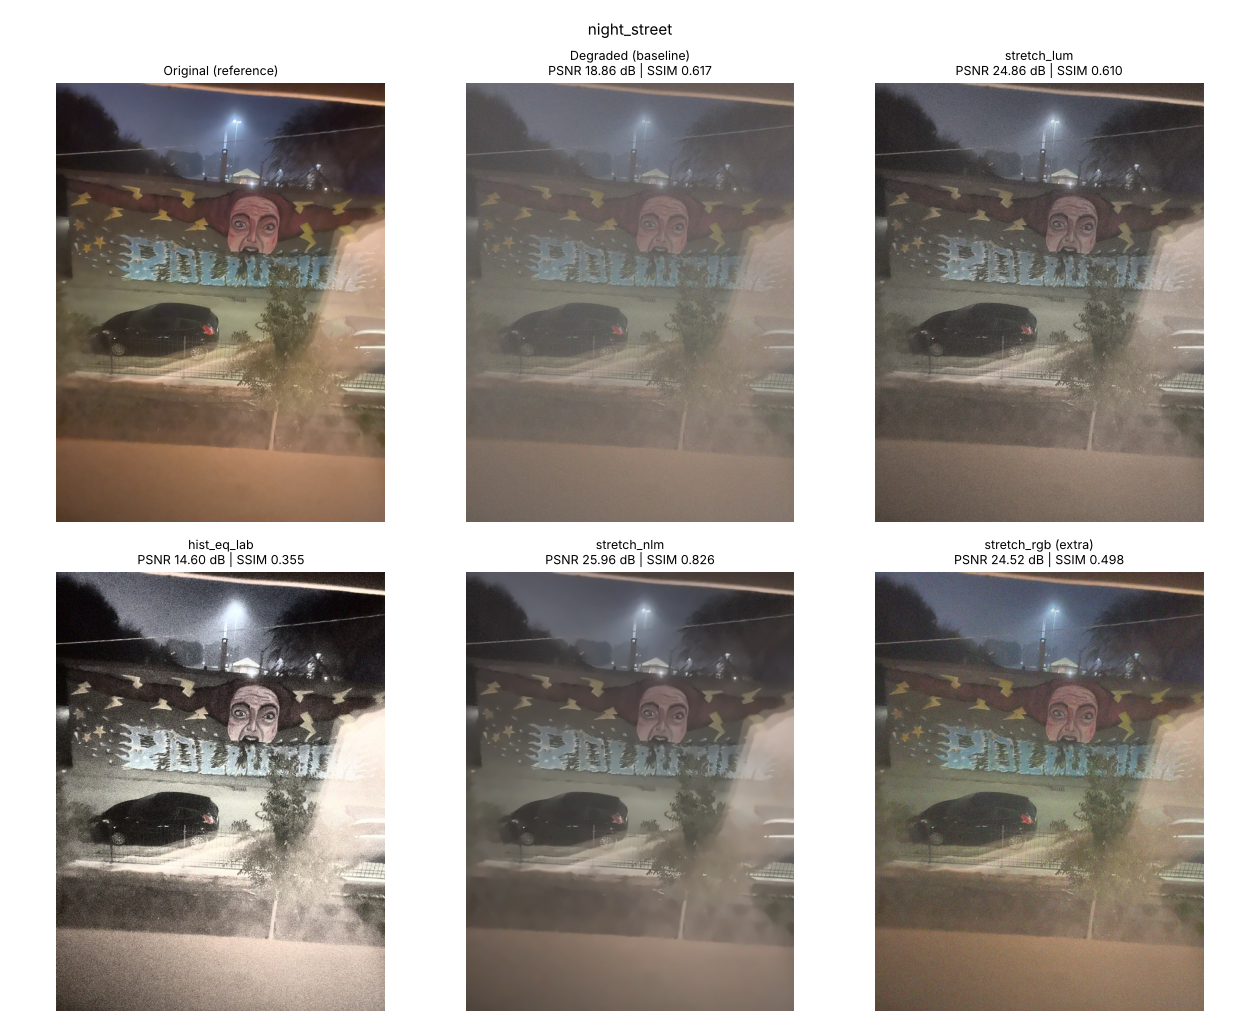
\includegraphics[width=0.84\linewidth]{night_street_comparison.png}
\caption{night\_street: same layout as Figure~\ref{fig:b1}.}\label{fig:ns}\end{figure}

\begin{table}[H]\centering\resizebox{\linewidth}{!}{\begin{tabular}{lccccc}\toprule Image & Baseline & Stretch (L) & Hist. eq. (L) & Stretch+NLM & Stretch RGB* \\ \midrule
board1 & 18.64 / 0.631 / 23.4 & 20.31 / 0.530 / 22.0 & 12.91 / 0.219 / 45.5 & 20.67 / 0.939 / 22.2 & 20.20 / 0.443 / 21.4 \\
board2 & 20.05 / 0.630 / 18.4 & 21.76 / 0.534 / 17.8 & 14.67 / 0.212 / 39.3 & 22.27 / 0.935 / 17.7 & 22.06 / 0.438 / 16.3 \\
board3 & 19.02 / 0.631 / 23.0 & 23.65 / 0.536 / 13.3 & 14.32 / 0.252 / 39.1 & 24.71 / 0.930 / 11.6 & 22.60 / 0.459 / 15.2 \\
night\_street & 18.86 / 0.617 / 24.5 & 24.86 / 0.610 / 12.0 & 14.60 / 0.355 / 38.4 & 25.96 / 0.826 / 10.6 & 24.52 / 0.498 / 12.2 \\
room\_dark & 17.96 / 0.569 / 27.1 & 22.62 / 0.496 / 15.6 & 15.60 / 0.293 / 33.7 & 23.57 / 0.862 / 14.0 & 21.66 / 0.392 / 17.5 \\
\midrule
\textbf{Mean} & \textbf{18.91 / 0.616 / 23.3} & \textbf{22.64 / 0.541 / 16.1} & \textbf{14.42 / 0.266 / 39.2} & \textbf{23.44 / 0.898 / 15.2} & \textbf{22.21 / 0.446 / 16.5} \\
\bottomrule\end{tabular}}
\caption{PSNR (dB) / SSIM / MAE against the original image (higher PSNR/SSIM and lower MAE are better). *Extra variant.}\label{tab:m}\end{table}

\begin{figure}[H]\centering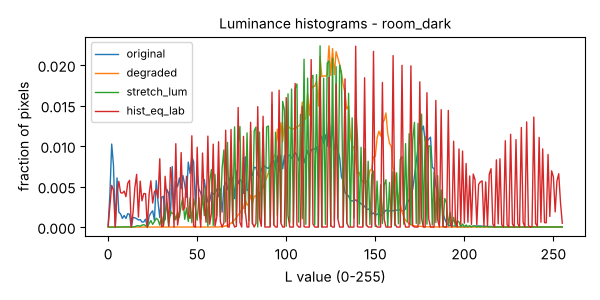
\includegraphics[width=0.55\linewidth]{room_dark_histograms.png}
\caption{Luminance (L) histograms for room\_dark. Stretching and equalization leave empty bins (comb pattern) because 8-bit values are spread over a wider range.}\label{fig:h}\end{figure}

\section*{4. Discussion}
\textbf{Stretching (luminance).} It raises the mean PSNR by about 3.7\,dB over the baseline (18.91 $\to$ 22.64\,dB) and brings back contrast, but the mean SSIM drops (0.616 $\to$ 0.541) because the gain also amplifies the noise, visible on flat areas (wall, floor, sky). Working on $L$ only keeps the hues; the per-RGB variant reaches a similar PSNR (22.21\,dB) but a lower SSIM (0.446) and shows colour casts (a greenish wall in board3, warm tint in room\_dark), because the three channels receive different gains.

\textbf{Histogram equalization} is the worst method (14.42\,dB, SSIM 0.266). Large, nearly uniform regions (white wall, dark floor, night sky) dominate the histogram, so equalization spreads tiny differences over the full range: noise is strongly amplified, bright regions are over-brightened and dark ones become grainy; since $a,b$ are unchanged while $L$ changes a lot, colours look washed out (desks in board1, sky in night\_street). Shadows and edges do become more visible, but the result looks unnatural.

\textbf{Stretch + NLM} gives the best numbers (23.44\,dB, SSIM 0.898) and the cleanest image. In night\_street (Fig.~\ref{fig:ns}) the mural and the car are clearly more visible than in the baseline with little noise; in room\_dark the noise on the floor disappears. The trade-off is smoothing: thin handwriting in board1 and the fine edges of the door in room\_dark become softer.

\textbf{Cases where numbers and appearance disagree.} (i) The SSIM of stretch+NLM is far higher than that of stretch alone (0.898 vs 0.541), partly because large flat regions dominate the images and are smoothed; this does not mean that details are better, since the handwriting is softer. (ii) In night\_street the stretch gains 6\,dB of PSNR over the baseline (18.86 $\to$ 24.86\,dB) while its SSIM stays the same (0.617 $\to$ 0.610): the image is clearly brighter and more contrasted, but the amplified noise cancels the structural gain. (iii) Percentile clipping (Table~\ref{tab:s}): stretching between the 1st and 99th percentiles looks more contrasted, but it saturates shadows and highlights and scores 6\,dB lower in PSNR than the min--max stretch (16.59 vs 22.64\,dB); a visually punchier image is not closer to the reference.

\begin{table}[H]\centering\small\begin{tabular}{rrrrr}\toprule $p_{low}$ (\%) & $p_{high}$ (\%) & PSNR (dB) & SSIM & MAE \\ \midrule
0 & 100 & 22.64 & 0.541 & 16.1 \\
0.1 & 99.9 & 20.41 & 0.460 & 21.8 \\
0.5 & 99.5 & 17.63 & 0.399 & 30.2 \\
1 & 99 & 16.59 & 0.368 & 34.2 \\
5 & 95 & 14.38 & 0.287 & 43.2 \\
\bottomrule\end{tabular}
\caption{Sensitivity of the luminance stretch to percentile clipping (mean over the five images).}\label{tab:s}\end{table}

\textbf{Preferred method.} For board1 and night\_street we prefer \textbf{stretch + NLM}: handwriting, shadow boundaries and the mural are easier to see than in the baseline, with much less noise than stretch alone. We would lower $h$ if the finest strokes were important.

\textbf{Limitations.} The degradation is a simple linear contrast loss plus Gaussian noise, and the references are not ideal images (they contain noise, glare and blur). Parameters were fixed for all images and not tuned per image, and five images are a small sample.

\section*{5. Reproducibility}
\texttt{python run\_experiment.py} runs the whole pipeline (Python 3.13, OpenCV, NumPy, scikit-image, matplotlib, pandas) and writes processed images, figures and \texttt{results/metrics.csv}. See the README for the structure and parameters.
\end{document}
